\subsection{AND}
	The AND gate implements logical conjunction ($\land$) from mathematical logic.
	Its operation can be represented as $\text{AND}(A, B) = A \cdot B$, where $A$ and $B$ are the input signals. \\
	The circuitry of an AND gate involves multiple transistors arranged in series. 
	For a two-input AND gate, two transistors are connected in series, as shown in Figure \ref{fig:AND_circuit}. \\
	If both inputs are high (1), both transistors conduct, creating a low-resistance path from the power supply to the output, resulting in a high output (1). 
	If either or both inputs are low (0), at least one of the transistors will be off, and the output will be pulled to a low state (0). 
    This behavior is consistent with the AND gate's truth table shown in Table \ref{tab:AND_table}. \\
	The symbol for the AND gate is shown in Figure \ref{fig:AND_sym}.

	\begin{figure}[H]
		\begin{minipage}{0.5\textwidth}
			\centering
			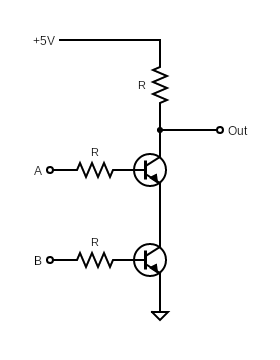
\includegraphics[width=0.8\textwidth]{figures/circuits/AND.png}
			\captionof{figure}{AND schematic circuit.}
			\label{fig:AND_circuit} 
		\end{minipage}
		\begin{minipage}{0.5\textwidth}
			\centering
			\captionof{table}{AND truth table.}
			\begin{tabular}{|c|c|c|}
				\hline
				Input A & Input B & Output \\
				\hline
				0 & 0 & 0 \\
				0 & 1 & 0 \\
				1 & 0 & 0 \\
				1 & 1 & 1 \\
				\hline
			\end{tabular}
			\label{tab:AND_table}
		\end{minipage}
	\end{figure}

	\begin{figure}[H]
	    \centering
	    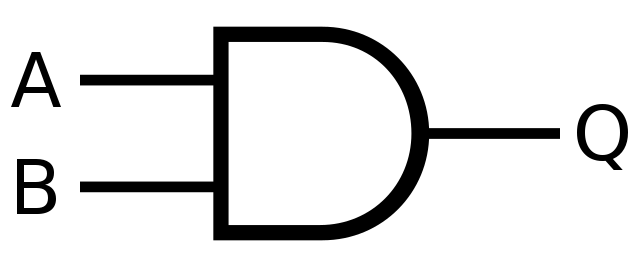
\includegraphics[width=0.3\textwidth]{figures/symbols/AND.png}
	    \caption{AND symbol.}
	    \label{fig:AND_sym} 
	\end{figure}

    \noindent
    The following photographs show the AND gate built in the laboratory and its behavior.
    \begin{figure}[H]
        \centering

        \begin{subfigure}{0.45\textwidth}
            \centering
            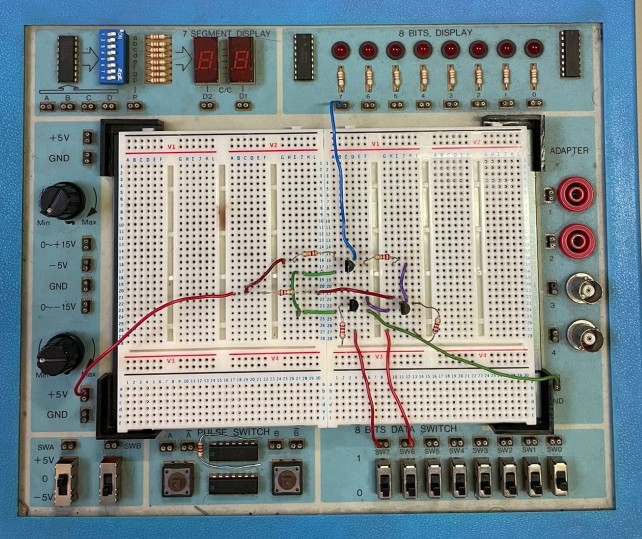
\includegraphics[width=\linewidth]{figures/photos/AND/00.png}
            \caption{A = 0, B = 0}
        \end{subfigure}
        \hfill
        \begin{subfigure}{0.45\textwidth}
            \centering
            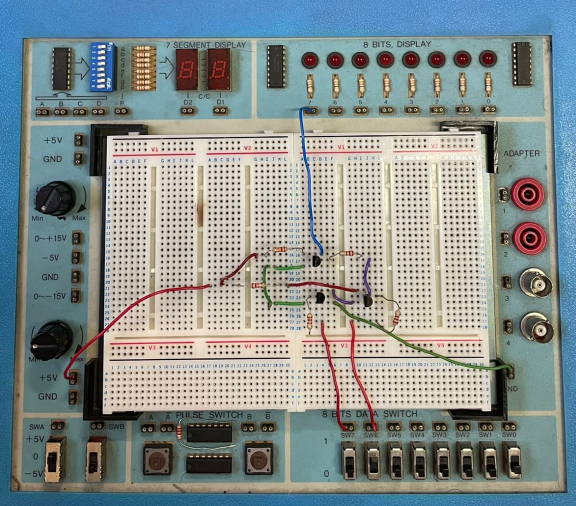
\includegraphics[width=\linewidth]{figures/photos/AND/01.png}
            \caption{A = 0, B = 1}
        \end{subfigure}

        \vspace{1cm} % Adjust vertical space between rows

        \begin{subfigure}{0.45\textwidth}
            \centering
            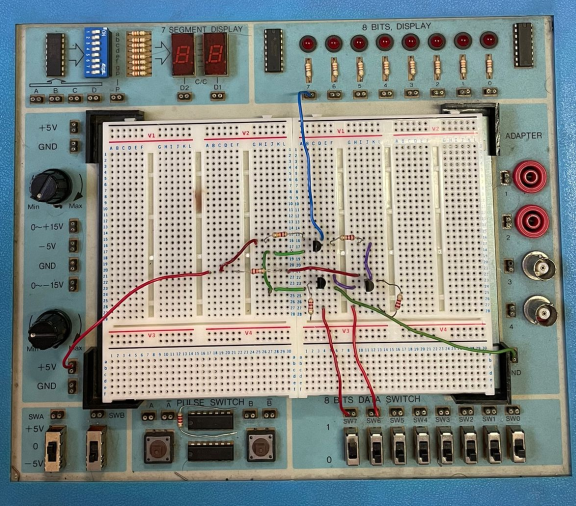
\includegraphics[width=\linewidth]{figures/photos/AND/10.png}
            \caption{A = 1, B = 0}
        \end{subfigure}
        \hfill
        \begin{subfigure}{0.45\textwidth}
            \centering
            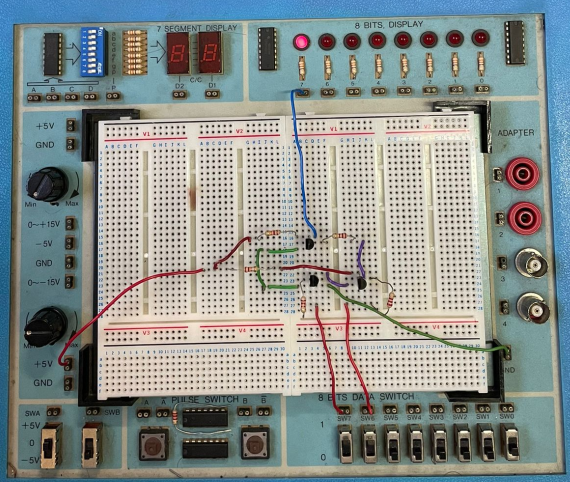
\includegraphics[width=\linewidth]{figures/photos/AND/11.png}
            \caption{A = 1, B = 1}
        \end{subfigure}

        \caption{AND gate constructed in the laboratory.}
        \label{fig:AND_photos}
    \end{figure}
